% IJCAI 2027 main track version (anonymous). Compile in paper: latexmk -pdf ijcai.tex
% Official call: https://2027.ijcai.org/ijcai-2027-call-for-papers-main-track/ (checked 2026-11-19)
% Style: https://www.ijcai.org/authors_kit (FormattingGuidelines-IJCAI-27.zip)
\documentclass{article}
\pdfpagewidth=8.5in
\pdfpageheight=11in
\usepackage{ijcai27}
\usepackage{times}
\usepackage{soul}
\usepackage{url}
\usepackage[hidelinks]{hyperref}
\usepackage[utf8]{inputenc}
\usepackage[small]{caption}
\usepackage{graphicx}
\usepackage{amsmath}
\usepackage{amssymb}
\usepackage{amsthm}
\usepackage{booktabs}
\usepackage{xcolor}
\usepackage[switch]{lineno}
\linenumbers
\urlstyle{same}

% The sections use natbib commands; map them to the IJCAI named style.
\newcommand{\citet}[1]{\citeauthor{#1}~\shortcite{#1}}
\newcommand{\citep}[1]{\cite{#1}}

\pdfinfo{
/TemplateVersion (IJCAI.2027.0)
}

\title{How Many Documents Cover a Corpus}
\author{Anonymous submission}

\begin{document}
\maketitle

\begin{abstract}
If we read 15 documents from a corpus, how much of the corpus have we seen? Researchers who study text read samples because they cannot analyze every document. A survey sample comes with a formula for its size and a margin of error, and a sample of text comes with neither. We measure what a sample has missed as the percentage of the corpus with no document of the same content in the sample, where we define two documents as the same content when their embeddings lie closer than a distance the researcher chooses. We estimate the missed percentage from the sample alone with a classical estimator built on what we call the isolation rate, the percentage of sampled documents with no other sampled document of the same content. To plan the size of a sample, we show that on most corpora we tested a larger sample and a looser definition of the same content trade against each other at a fixed rate. The rate is set by the intrinsic dimension of the corpus, the number of independent ways in which its documents differ in meaning. This rate gives a sample size formula. In 77 of 83 tests, each a combination of corpus, target and distance, the sample actually needed fell between two thirds and one and a half times the formula's answer. A pilot of 2{,}000 documents shows in advance whether the formula can be trusted for a given corpus. Two large language models judged pairs of documents to tell which distance means the same specific content and which means the same topic.
\end{abstract}

\section{Introduction}

Researchers who study large collections of text work with samples, because the collections contain more text than people or models can process. An annotation team labels as many posts as its budget pays for. A large language model takes in only as much text as fits in its context window. Qualitative researchers stop interviewing at saturation, when new interviews stop adding new themes, which the literature places at about 9 to 17 interviews \citep{guest2006,hennink2022}. In each case a budget or a convention sets the size of the sample. If we read 15 posts from a corpus of 10{,}000, can we be sure we basically understand the corpus? Would 100 or 1{,}000 posts be enough?

Survey research answers the same question for an estimate about a population. Before the survey, a sample size formula tells the designer how many respondents a target margin of error requires \citep{cochran1977,kish1965}. After the survey, the margin of error tells the reader how far the estimate may lie from the population value. A sample of a corpus comes with neither. The question a reader of such a sample has in mind is how much of the corpus has a similar document among the documents read. This paper builds an estimate of that percentage and a sample size formula for it.

A text encoder turns each document into an embedding, a list of numbers, so that documents with similar meaning have embeddings close together. We define two documents as the same content when the cosine distance between their embeddings is smaller than a resolution $r$ chosen by the researcher. A researcher who needs the same specific claim chooses a small $r$, and one who needs only the same topic chooses a larger one. To give $r$ a meaning in content, two large language models judged pairs of documents at a range of distances.

With $r$ fixed, a corpus document is missed when no sampled document lies within $r$ of it. The missing mass is the percentage of the corpus that is missed. A researcher who holds only the sample cannot count the missed documents directly. Good and Turing faced the same problem with words, and estimated the probability that the next word of a text is one not yet seen from the words seen exactly once \citep{good1953}. \citet{maurer2022missing} extended this estimator from words to distances. Its input is what we call the isolation rate $G$, the percentage of sampled documents with no other sampled document within $r$. A sample of $n$ documents from a corpus of $N$ estimates the missing mass as $G\,(1 - n/N)$, where $1 - n/N$ is the finite population correction of survey sampling. Maurer develops the estimator in theory, and in a search of the literature in 2026 we found no work that applies it to text.

How fast the missing mass falls as the sample grows follows from a classical geometric result about nearest neighbors among randomly scattered points \citep{penrose2003rgg,levina2005}. The intrinsic dimension $d$ of a corpus is the number of independent ways in which its documents differ in meaning. We find that, on most of the corpora we tested, any two samples with the same product $n r^{d/2}$ leave the same percentage of their documents isolated. A larger sample and a looser resolution therefore trade against each other at a fixed rate set by $d$. Under this law, halving $r$ requires $2^{d/2}$ times as many documents, which for $d = 26$ is about 8{,}000 times as many. The dimension $d$ does for a corpus what the variance does for a survey population. A population with a larger variance needs more respondents for the same margin of error, and a corpus with a larger $d$ needs more documents for the same resolution.

We test the estimate and the formula on synthetic data with a known answer and on ten real corpora: three Reddit forums, five slices of 2020 tweets about the United States Census, and random samples of English posts from Truth Social and Bluesky in 2024. The paper makes four contributions.
\begin{enumerate}
\item A measure of what a sample of text has missed, the missing mass at a resolution chosen by the researcher, which the sample alone estimates through the isolation rate and the finite population correction of survey sampling.
\item A sample size formula, obtained by solving the law for $n$, with a pilot test that tells whether the formula can be trusted on a given corpus.
\item A way to give the resolution $r$ a meaning in content, by having large language models judge pairs of documents.
\item A measurement of how much of a corpus a sample chosen by $k$-means covers against a random sample of the same size. The chosen sample covers far more of the corpus on corpora that repeat themselves.
\end{enumerate}

\section{Background}

\subsection{The missing mass of a sample of categories}

The missing mass of a sample was first estimated for samples of categories, such as words in a text or species in a forest. A sample of $n$ draws covers the categories it contains, and the missing mass is the total proportion of the population that belongs to categories the sample never saw. \citet{good1953} showed that $f_1/n$, the proportion of draws whose category appears only once, estimates the missing mass with little bias. The intuition is that a category seen once is the kind of category that could easily have been missed. Ecologists built a whole sampling theory on the same idea, because no field survey finds every species and the surveyor must decide when to stop. \citet{chao2012coverage} wrote the coverage a survey would reach after $m$ more draws as a formula in $n$ and the counts of species seen once and twice, so that a survey can be planned to stop at a target coverage. These estimators have been applied to text a few times \citep{tran2017,hajic2025}. In these studies an item belongs to a discrete category and two items either match or do not. Documents rarely fall into such categories. Two posts can make the same point in different words, and two posts with many words in common can make opposite points.

\subsection{The missing mass with distances between items}

\citet{maurer2022missing} removed the need for categories. He works in any space with a distance $\delta(\cdot, \cdot)$ between items. For a sample $X_1, \dots, X_n$ and a distance $r$, the missing mass is the probability that a new item lies farther than $r$ from every item in the sample. His estimator is
\begin{equation}
G(X, r) = \frac{1}{n}\,\big|\{k : \delta(X_k, X_i) > r \text{ for all } i \neq k\}\big| ,
\label{eq:G}
\end{equation}
the proportion of sampled items that have no other sampled item within $r$. When items are categories, $G$ is exactly Good and Turing's $f_1/n$. Maurer proved that $G$ overstates the missing mass by at most $1/n$ on average. His paper is theory, and it contains no data, no embeddings and no statement about how $G$ changes as the sample grows.

That change is described by a classical result about nearest neighbors. Suppose items are drawn from a density $f$ on a set of dimension $d$. Then the probability that an item at $x$ has no other item within Euclidean distance $r$ among $n$ draws is close to $\exp(-n f(x)\, v_d\, r^{d})$, where $v_d$ is the volume of a ball of radius 1 in $d$ dimensions \citep{evans2002,penrose2003rgg}. The same result is the basis of the estimators of intrinsic dimension proposed by \citet{levina2005} and \citet{facco2017twonn}, which work backward from nearest neighbor distances to $d$. We use it forward, to predict how $G$ falls as $n$ grows.

\subsection{Diversity measures and stopping rules}

Several measures describe how spread out a set of embedded documents is, such as the Vendi score \citep{friedman2023vendi} and the precision and recall of \citet{kynkaanniemi2019}. Each of these measures describes the sample in hand or compares two samples. None predicts what a larger sample would cover. Where a sample size for text is set on purpose at all, it is set by a stopping rule. Qualitative researchers stop interviewing at saturation \citep{guest2006,hennink2022}, and TopicGPT stops when 200 further documents add no new topic \citep{pham2024topicgpt}. Each of these studies observes one coverage curve and stops on it. None can say, before reading, where the curve will flatten for a new corpus. The present paper gives the curve a parameter, the intrinsic dimension $d$, and an estimator that a researcher can compute from the sample.

\section{Method}

\subsection{The missing mass of a corpus sample}

A corpus is a finite set of $N$ documents $x_1, \dots, x_N$. We embed each document with a fixed encoder, scale each embedding to length 1, and measure the distance between two documents by the cosine distance of their embeddings. A sample $S$ is a set of $n$ documents drawn at random without replacement. The user chooses a resolution $r$, and we define two documents within $r$ of each other as the same content for the purpose at hand. The quantity we estimate is the missing mass of the sample at resolution $r$,
\begin{equation}
M(S, r) = \frac{1}{N}\,\big|\{j : \delta(x_j, x_i) > r \text{ for all } i \in S\}\big| ,
\end{equation}
the proportion of corpus documents that have no sampled document within $r$. If $M = 0.6$, then 60\% of the corpus consists of documents for which the sample holds no document with the same content, and a summary or an annotation built from the sample can say nothing specific about them. Computing $M$ requires the whole embedded corpus. The estimator $G$ of Equation~\ref{eq:G} needs only the sample. We write $G(n, r)$ for its value on a sample of $n$ documents. In our experiments the whole corpus is available, so we can check every estimate against the true $M$.

\subsection{The collapse law}

Suppose the embedded documents lie close to a set of intrinsic dimension $d$, far smaller than the 768 or 4{,}096 coordinates of an embedding. Around a document $x$, the proportion of the corpus that lies within Euclidean distance $\rho$ is then about $c(x)\, \rho^{d}$, where $c(x)$ is larger where documents are densely packed. Between embeddings of length 1, the cosine distance is half the squared Euclidean distance, so the proportion of the corpus within cosine distance $r$ of $x$ is about $c(x)\, r^{d/2}$. The chance that none of $n$ sampled documents falls within $r$ of $x$ is about $\exp(-c(x)\, n\, r^{d/2})$. Averaging over documents gives
\begin{equation}
\mathbb{E}\, G(n, r) \approx \mathbb{E}_{x}\big[\exp(-c(x)\, n\, r^{d/2})\big] = \mathcal{L}_{c}(n\, r^{d/2}),
\end{equation}
where $\mathcal{L}_{c}$ is the Laplace transform of the distribution of $c$ over documents. Whatever the density looks like, two samples with the same product $n r^{d/2}$ have the same expected $G$, as long as one $d$ holds across the resolutions of interest. We call this the collapse law, because curves of $G$ against $n$ at different resolutions fall onto one curve when they are plotted against $n r^{d/2}$. On the synthetic manifolds, where we use Euclidean distance, the product is $n r^{d}$.

Real corpora mix dense regions, where many documents say similar things, with sparse regions, where documents are unusual, and the curve then falls more slowly than a pure exponential. We describe the shape by a stretched exponential, $G = \exp(-(\kappa\, n\, r^{d/2})^{b})$ with $0 < b \le 1$. Taking logarithms twice turns this into a straight line,
\begin{equation}
\log\big(-\log G(n, r)\big) = a + b \log\big(n\,r^{d/2}\big),
\label{eq:collapse}
\end{equation}
which we fit by least squares. We estimate $d$ beforehand with the TwoNN estimator of \citet{facco2017twonn}, which uses, for every document, the ratio of the distance to its second nearest neighbor to the distance to its first, averaged over five pilot samples of 2{,}000 documents. To fit $a$ and $b$, we draw five independent samples at each of eleven sample sizes from 100 to 7{,}000 (no more than $0.7N$), and compute $G$ at twelve resolutions spaced evenly on a log scale between the 5th and the 99th percentile of the nearest neighbor distances in a pilot. Only cells with $0.02 < G < 0.98$ enter the fit. As a check on $d$ that does not use TwoNN, we also fit $\log(-\log G)$ on $\log n$ and $\log r$ as two separate regressors, so that twice the ratio of their coefficients is a second estimate of $d$.

\subsection{The sample size formula}

Solving Equation~\ref{eq:collapse} for $n$ gives the sample size at which the isolation rate at resolution $r$ falls to a target $\varepsilon$,
\begin{equation}
n^{*}(\varepsilon, r) = \left(\frac{\log(1/\varepsilon)}{e^{a}}\right)^{1/b} r^{-d/2} .
\label{eq:nstar}
\end{equation}
For example, $\varepsilon = 0.2$ asks for a sample in which at most 20\% of the documents are isolated, which, by the argument of Good and Turing, is a sample that leaves about 20\% of the corpus unseen. The corpus enters the formula through three numbers, $d$, $a$ and $b$, and all three can be estimated from a pilot.

\subsection{The finite population correction}

$G$ estimates the missing mass of the process that generated the corpus, as if new documents kept arriving. When the target is the corpus itself, the $n$ sampled documents are part of the corpus, and each of them has something like it in the sample, namely itself. Each of the other $N - n$ documents is isolated from the sample with a probability close to $G$. The missing mass of the corpus is therefore
\begin{equation}
\hat M(n, r) = G(n, r)\,\big(1 - n/N\big).
\label{eq:fpc}
\end{equation}
The factor $1 - n/N$ is the one survey sampling calls the finite population correction \citep{groves2009survey}.

\subsection{A pilot test for the law}

The collapse law assumes that one intrinsic dimension holds across the resolutions of interest, and a researcher needs to know whether that holds before drawing the sample. We fit Equation~\ref{eq:collapse} on subsamples of a pilot of 2{,}000 documents with up to 750 documents, and we compute how much of the variance of $\log(-\log G)$ the fit explains on subsamples of 1{,}000 to 2{,}000 documents, which it did not see. A corpus passes when this pilot $R^2$ is at least 0.95. To check the pilot test, we also fit the law on samples of up to 1{,}000 documents from the whole corpus and evaluate it on samples of up to 7{,}000.

\subsection{Calibrating the resolution with judgments of content}
\label{sec:rcalm}

For each real corpus, we drew about 40 pairs of documents in each of ten bins of distance between 0 and 1. A large language model read each pair and judged whether the two documents are about the same specific content (the same claim, question, event or story), about the same general topic, or unrelated. We call $r_{\mathrm{same}}$ the distance at which the percentage of pairs judged the same content crosses one half, and $r_{\mathrm{topic}}$ the distance at which the percentage judged the same content or the same topic crosses one half. Two models judged every pair, Qwen3.8-27B and Gemma-4-31B-it.

\subsection{Choosing the documents to read}
\label{sec:design}

A researcher who holds the whole corpus can embed it and choose which $n$ documents to read. We take the $k$-means design from work that picks data for a model to learn from \citep{chang2021training,yuan2020coldstart,hacohen2022active,zhang2023autocot}. The researcher divides the corpus into $n$ groups of similar documents \citep{lloyd1982} and reads the document nearest the center of each group. We measure how much of the corpus the chosen documents cover, against a random sample of the same size.

\section{Data}
\label{sec:data}

The synthetic data come in two families. The Gaussian manifolds place 20{,}000 points on a random subspace of dimension $d \in \{2, 4, 8\}$ inside a space of 64 dimensions, so the true intrinsic dimension is known. The Zipf mixture draws 20{,}000 points around 200 topic centers, with topic sizes that follow a Zipf distribution, so the topic of every point is known.

Three forum corpora from Reddit hold 10{,}000 documents each: AskDocs holds medical questions, Trump holds posts about the 2020 presidential election, and TIFU holds personal stories told in the first person. We embed them twice, with GTR-T5-base \citep{ni2022gtr} on three random samples of the source, and with Qwen3-Embedding-8B \citep{qwen3embedding2025}. Five corpora come from a 2020 collection of tweets about the United States Census, each a slice selected by a keyword (citizens, trump, covid, illegal) or, for the random slice, drawn without a keyword, with between 7{,}610 and 30{,}136 tweets. Two corpora are random samples of 50{,}000 English posts each from Truth Social and Bluesky, written between May and December 2024 and collected through the platforms' public interfaces. These seven corpora are embedded with Qwen3-Embedding-8B. With the four synthetic sets, this makes the seventeen pairs of corpus and encoder of Table~\ref{tab:collapse}. The analysis uses only embeddings and statistics computed over whole corpora, and no post or account is quoted or identified.

\section{Results}

\subsection{The isolation rate tracks the true coverage}

In the synthetic Zipf mixtures every document belongs to a known topic, so we know exactly which percentage of the topics a sample has covered. Over four settings of the mixture, three random seeds and eleven sample sizes from 50 to 5{,}000, the coverage $1 - G$ at a resolution of half the median distance between documents in a pilot follows the true topic coverage closely. The rank correlation is $\rho = 0.968$, and $1 - G$ is off by 2.9 percentage points on average. At smaller resolutions the agreement falls away, because two documents of the same topic often lie farther apart than $r$. The resolution must therefore match the question being asked of the sample.

\subsection{The isolation rate collapses on $n r^{d/2}$}
\label{sec:collapse}

Table~\ref{tab:collapse} reports the fit of Equation~\ref{eq:collapse} on 17 pairs of corpus and encoder, and Figure~\ref{fig:collapse} shows six of them. On ten pairs the law holds: the three synthetic manifolds, AskDocs and TIFU under both encoders, the random slice of the Census tweets, Truth Social and Bluesky. On these ten, a fit on samples of up to 1{,}000 documents explains 92\% or more of the variance of $\log(-\log G)$ in samples of up to 7{,}000 documents. In terms of $G$ itself, the law predicts the isolation rate of the largest sample with an average error between 1.5 and 4.2 percentage points on these ten pairs. A researcher who has drawn a few hundred documents can thus predict from them alone what percentage of a sample twenty times larger will be isolated, at every resolution at once.

For AskDocs and TIFU, the points of all colours in Figure~\ref{fig:collapse} lie on one curve once the horizontal axis is $n r^{d/2}$, so that a larger sample and a looser resolution are interchangeable. For Trump and for the Zipf mixture, each colour traces its own curve, and no single $d$ brings them together. The second estimate of $d$, from the separate coefficients on $\log n$ and $\log r$, differs from the TwoNN estimate by at most 19\% on the ten passing pairs, and by 27\% to 46\% on the seven failing pairs.

The law also predicts better than the two obvious alternatives, both fitted on the same samples of up to 1{,}000 documents. A separate curve in $n$ at each resolution, which needs no $d$, has 1.5 to 3.8 times the average error of the law on nine of the ten passing pairs. The law wins because it pools the information from all resolutions through one $d$. The extrapolation of \citet{chao2012coverage}, the standard ecological tool, run within its recommended range, has 2 to 9 times the average error of the law on the passing pairs.

\begin{figure*}[t]
\centering
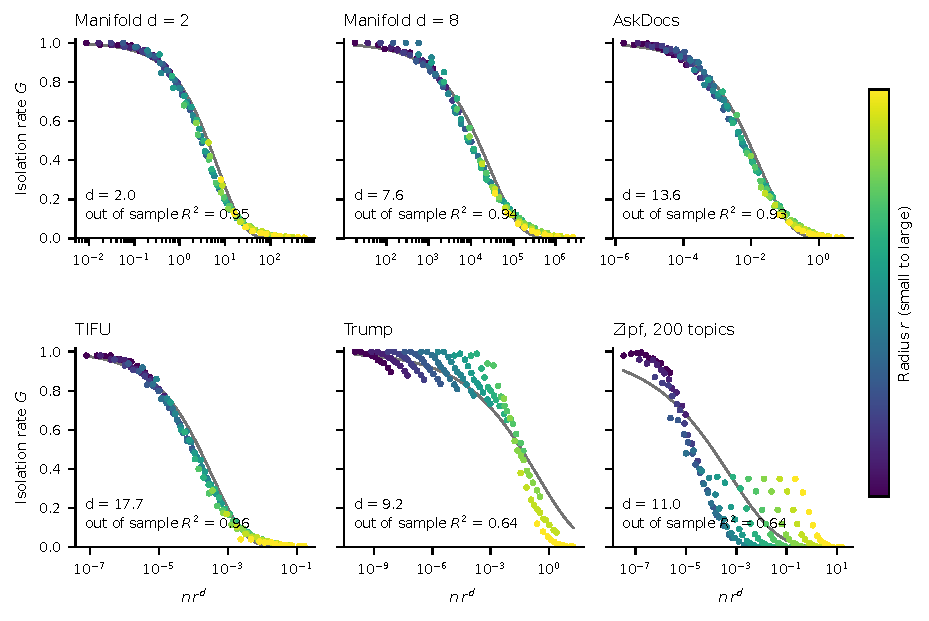
\includegraphics[width=\textwidth]{figures/collapse.pdf}
\caption{Isolation rate $G$ against $n r^{d/2}$ (log scale; $n r^{d}$ on the manifolds, which use Euclidean distance), one panel per corpus, with the GTR encoder for the three forum corpora. Each point is one sample size at one resolution, and the colour gives the resolution, from the 5th (dark) to the 99th (light) percentile of the nearest neighbor distances in a pilot. Where the law holds (the synthetic manifolds, AskDocs, TIFU), points from all resolutions fall on one curve. Where it fails (Trump, the Zipf mixture), the points of each resolution form their own curve. The grey line is the fit of Equation~\ref{eq:collapse} on samples of up to 1{,}000 documents. Each panel gives $d$ and the full out of sample $R^2$ from Table~\ref{tab:collapse}.}
\label{fig:collapse}
\end{figure*}

\begin{table*}[t]
\centering
\small
\setlength{\tabcolsep}{5pt}
\begin{tabular}{llrrrrrrrr}
\toprule
Corpus & Encoder & $N$ & $d$ (sd) & $d$, ratio & $b$ & $R^2$ pilot & $R^2$ full & error, law & error, per resolution \\
\midrule
AskDocs & Qwen3 & 10{,}000 & 25.5 (0.78) & 24.4 & 0.54 & 0.98 & 0.99 & 0.015 & 0.057 \\
Truth Social & Qwen3 & 50{,}000 & 25.3 (0.30) & 28.9 & 0.43 & 0.98 & 0.98 & 0.025 & 0.053 \\
Census random & Qwen3 & 7{,}610 & 25.7 (0.78) & 24.8 & 0.27 & 0.98 & 0.97 & 0.040 & 0.025 \\
Manifold $d{=}2$ & none & 20{,}000 & 2.0 (0.05) & 2.4 & 0.80 & 0.97 & 0.96 & 0.027 & 0.065 \\
TIFU & Qwen3 & 10{,}000 & 27.3 (0.70) & 26.8 & 0.53 & 0.98 & 0.96 & 0.039 & 0.086 \\
Bluesky & Qwen3 & 50{,}000 & 32.0 (1.38) & 30.4 & 0.42 & 0.98 & 0.96 & 0.037 & 0.056 \\
TIFU & GTR & 10{,}000 & 36.5 (0.66) & 38.1 & 0.50 & 0.97 & 0.95 & 0.040 & 0.070 \\
Manifold $d{=}8$ & none & 20{,}000 & 8.0 (0.21) & 8.1 & 0.62 & 0.97 & 0.95 & 0.042 & 0.081 \\
AskDocs & GTR & 10{,}000 & 27.3 (0.71) & 27.1 & 0.51 & 0.98 & 0.95 & 0.042 & 0.087 \\
Manifold $d{=}4$ & none & 20{,}000 & 4.0 (0.16) & 4.3 & 0.72 & 0.96 & 0.92 & 0.036 & 0.091 \\
\midrule
Census illegal & Qwen3 & 17{,}202 & 22.8 (0.66) & 15.0 & 0.26 & 0.93 & 0.85 & 0.026 & 0.053 \\
Census covid & Qwen3 & 17{,}837 & 21.3 (0.80) & 14.4 & 0.30 & 0.85 & 0.79 & 0.045 & 0.073 \\
Trump & Qwen3 & 10{,}000 & 17.9 (1.02) & 10.5 & 0.26 & 0.90 & 0.78 & 0.045 & 0.075 \\
Census trump & Qwen3 & 30{,}136 & 18.0 (1.68) & 12.6 & 0.26 & 0.87 & 0.78 & 0.043 & 0.056 \\
Census citizens & Qwen3 & 7{,}849 & 18.1 (0.48) & 13.2 & 0.27 & 0.76 & 0.73 & 0.043 & 0.058 \\
Trump & GTR & 10{,}000 & 17.9 (0.97) & 10.4 & 0.27 & 0.79 & 0.63 & 0.054 & 0.069 \\
Zipf, 200 topics & none & 20{,}000 & 22.7 (0.70) & 12.9 & 0.21 & 0.66 & 0.62 & 0.136 & 0.026 \\
\bottomrule
\end{tabular}
\caption{The collapse law on 17 pairs of corpus and encoder, sorted by the full out of sample $R^2$. Pairs above the line pass the pilot test. $d$: intrinsic dimension by TwoNN with Euclidean distance between unit embeddings (Euclidean distance on the manifolds), mean and standard deviation over five pilots of 2{,}000 documents (over three samples of the source for the GTR forum corpora). $d$, ratio: the second estimate of $d$, from the ratio of the coefficients on $\log r$ and $\log n$. $b$: shape exponent of Equation~\ref{eq:collapse}, fitted on samples of up to 1{,}000 documents. $R^2$ pilot: proportion of variance explained on subsamples of 1{,}000 to 2{,}000 documents of one pilot, by a fit on subsamples of up to 750. $R^2$ full: proportion of variance explained on samples of up to 7{,}000 documents, by a fit on samples of up to 1{,}000. Error, law and error, per resolution: average error in predicting $G$ at the largest sample, for the collapse law and for a separate curve in $n$ at each resolution.}
\label{tab:collapse}
\end{table*}

\begin{table*}[t]
\centering
\small
\setlength{\tabcolsep}{4pt}
\resizebox{\textwidth}{!}{%
\begin{tabular}{llcrrrcrrr}
\toprule
 & & \multicolumn{4}{c}{Qwen3.8-27B} & \multicolumn{4}{c}{Gemma-4-31B} \\
\cmidrule(lr){3-6}\cmidrule(lr){7-10}
Corpus & Diag. & $r_{\mathrm{same}}$ [90\%] & $n$ (\%) & pred. & interval & $r_{\mathrm{same}}$ [90\%] & $n$ (\%) & pred. & interval \\
\midrule
TIFU & pass & $\le$.05 [.05, .10] & 4{,}997 (50\%) & 50\% & 50\% & .08 [.05, .10] & 4{,}997 (50\%) & 50\% & 50\% \\
AskDocs & pass & .15 [.13, .16] & 4{,}953 (50\%) & 50\% & 50\% & .17 [.16, .19] & 4{,}923 (49\%) & 50\% & 49\% \\
Truth Social & pass & .16 [.15, .18] & 21{,}942 (44\%) & 48\% & 42\% to 45\% & .18 [.17, .20] & 20{,}610 (41\%) & 45\% & 39\% to 43\% \\
Cens.\ random & pass & .12 [.10, .18] & 3{,}352 (44\%) & 48\% & 35\% to 45\% & .28 [.26, .29] & 532 (7.0\%) & 9.2\% & 3.9\% to 11\% \\
Cens.\ covid & fail & .20 [.19, .21] & 3{,}356 (19\%) & 20\% & 17\% to 22\% & .29 [.22, .30] & 279 (1.6\%) & 1.7\% & 0.6\% to 14\% \\
Cens.\ citizens & fail & .23 [.20, .26] & 370 (4.7\%) & 4.9\% & $<$1.3\% to 10\% & .35 [.32, .38] & $<$100 ($<$1.3\%) & 0.1\% & $<$1.3\% \\
Trump (forum) & fail & .24 [.22, .26] & 442 (4.4\%) & 4.1\% & 2.2\% to 10\% & .31 [.31, .33] & $<$100 ($<$1.0\%) & 0.4\% & $<$1.0\% \\
Cens.\ trump & fail & .24 [.17, .25] & 604 (2.0\%) & 1.6\% & 1.0\% to 18\% & .31 [.29, .33] & $<$100 ($<$0.3\%) & 0.2\% & $<$0.3\% \\
Cens.\ illegal & fail & .28 [.25, .29] & $<$100 ($<$0.6\%) & 0.3\% & $<$0.6\% & .30 [.29, .32] & $<$100 ($<$0.6\%) & 0.1\% & $<$0.6\% \\
\bottomrule
\end{tabular}}
\caption{The distance that means the same content, and the random sample after which half of the corpus has a document with the same content in the sample. $r_{\mathrm{same}}$: distance at which half of the judged pairs are about the same specific content, with a 90\% interval from resampling the pairs. $n$ (\%): the sample size, measured on the whole corpus, as a count and as a percentage of the corpus. The percentage can never exceed 50\%, because the sampled half of a corpus is covered by itself. pred.: the percentage predicted from a pilot of 2{,}000 documents alone. interval: the measured percentage at the two ends of the 90\% interval of $r_{\mathrm{same}}$. $<$100: reached before the smallest sample of 100. $\le$: the crossing lies at the first bin, and 32\% of resamples find no crossing. Bluesky passes the pilot test but has no crossing, although 26\% (Qwen3.8) and 34\% (Gemma) of resamples find one. Truth Social and Bluesky are samples of 50{,}000 posts, and their percentages describe corpora of that size. Diag.: the pilot test of Section~\ref{sec:diag}.}
\label{tab:rcal}
\end{table*}

\subsection{The sample size formula}
\label{sec:nstar}

To test the formula, we treated each pair of corpus and encoder as a researcher would. We fitted Equation~\ref{eq:collapse} on samples of up to 1{,}000 documents, and Equation~\ref{eq:nstar} gave the sample size $n^{*}$ needed to bring the isolation rate down to 30\%, 20\% or 10\% at each resolution. We kept every case in which the true sample size lies beyond 1{,}000 documents, so that each case is a genuine prediction, and compared $n^{*}$ with the sample size at which $G$ actually reached the target in repeated draws. The ten passing pairs give 83 such cases.

On the ten passing pairs, the formula comes close in 77 of 83 cases, in the following sense: the sample that actually reached the target held between two thirds of $n^{*}$ and one and a half times $n^{*}$. A formula answer of 1{,}500 documents thus meant an actual need between 1{,}000 and 2{,}250 documents. When $a$ and $b$ are fitted inside one pilot of 2{,}000 documents, as a user would fit them, the formula comes close in 76 of 83 cases. On the seven failing pairs it comes close in only 10 of 23 cases. Refitting on 50 pilots gives intervals for $n^{*}$ with a median width of 19\% of $n^{*}$, which contain the true sample size in only 21\% of the cases, so the error of $n^{*}$ comes mostly from the shape of the law. We therefore report $n^{*}$ with the band observed in the tests, two thirds to one and a half times $n^{*}$, which contains the true sample size in 93\% of the cases on passing corpora.

\subsection{The pilot test}
\label{sec:diag}

The ten passing pairs reach a pilot $R^2$ of 0.96 or more, and the seven failing pairs reach at most 0.93 (Table~\ref{tab:collapse}). A threshold of 0.95 on the pilot therefore sorts every pair the same way as the full test on the whole corpus. We chose the threshold on these corpora, so it should be confirmed on others. The law should fail when the effective dimension of a corpus changes with the resolution. On Trump, clusters with a dimension near 2 hold slogans, short posts repeated in many small variations, and clusters with a dimension near 16 hold discussion. At small resolutions the isolated documents come mainly from one kind of cluster, and at large resolutions mainly from the other, so no single $d$ lines up the curves.

\subsection{The finite population correction}
\label{sec:fpc}

We compared $G$ and $G\,(1 - n/N)$ with the true missing mass $M$ on the eight forum and Census corpora under Qwen3, at sampling fractions from 1\% to 70\% of the corpus and three resolutions, 144 cases in all. Without the correction, $G$ is off by 11 percentage points on average and by as much as 49 points. With it, the estimate is off by 1.2 points on average and by at most 11 points. On random samples of 15 documents at the calibrated distances of Section~\ref{sec:rcal}, $G\,(1-n/N)$ lies within 6 percentage points of the true missing mass on every corpus, and its error averages 1.6 percentage points.

\subsection{Calibrated resolutions}
\label{sec:rcal}

On every corpus, the percentage of pairs that the judge calls the same content falls steadily as the distance grows. Where it crosses one half, however, depends on the corpus (Table~\ref{tab:rcal}). Under Qwen3.8, $r_{\mathrm{same}}$ lies at 0.05 or below on TIFU and reaches 0.28 on the Census tweets that contain the word ``illegal''. Long personal stories differ in their details even when their embeddings are close, while short posts that repeat a slogan remain the same content at a larger distance. The two judges give the same label to 71\% of pairs (Cohen's $\kappa = 0.55$), and Gemma's crossing lies farther out on every corpus. The judge is therefore part of the definition of $r$, and a user should report it together with the encoder.



Table~\ref{tab:rcal} also gives the random sample after which half of each corpus has a document with the same content in the sample. In a corpus in which no two documents share content, the sample covers only itself, so reaching this target takes exactly half of the corpus. On the Trump forum and the Census slices with the keywords citizens, trump and illegal, which repeat a few claims, at most 604 documents reach the target under either judge. On AskDocs, TIFU and Truth Social the sample must hold between 41\% and 50\% of the corpus. For these corpora, a sample covers what it contains and little more. The collapse law fitted on one pilot of 2{,}000 documents puts every corpus in the same group as the measurement.

\subsection{Choosing the documents to read}
\label{sec:design-results}

Choosing documents with the whole corpus embedded covers far more than random sampling wherever the corpus repeats itself. A random sample of 15 tweets from the Census illegal slice misses 62\% of the slice at the content level, and the same number of tweets chosen by $k$-means misses 33\%. On the Trump forum, $k$-means lowers the missing mass of a sample of this size from 88\% to 64\%. Where documents rarely have the same content as any other document, no choice of documents helps. On AskDocs at the content level, a random sample of 15 questions and a $k$-means sample of the same size both miss 99.8\% of the forum. The isolation rate $G$ of a random pilot of 100 documents predicts how much of the missing mass $k$-means removes (Spearman rank correlation $-0.90$ over 17 combinations of corpus and level). The supplementary material reports the full comparison.

\section{Discussion}

Whether 15 documents are enough to understand a corpus depends on the corpus and on the level of content the reader needs. On a repetitive corpus, 15 documents show nearly every topic, because the corpus returns again and again to a limited number of claims. At the level of specific content, 15 random documents covered no corpus we studied. When a study needs a sample size for a target, a researcher can fit the law of Equation~\ref{eq:collapse} on a pilot of 2{,}000 documents, apply the pilot test of Section~\ref{sec:diag}, and use the formula of Equation~\ref{eq:nstar} only when the corpus passes that test. With the sample drawn, $G\,(1 - n/N)$ estimates the missing mass from the sample alone.

The measure follows survey sampling at three points. The first is the finite population correction. A sampled document covers itself, so the estimate multiplies $G$ by $1 - n/N$, the factor survey sampling uses for a sample drawn from a finite population \citep{cochran1977}. The second is the intrinsic dimension $d$, which plays the role of the variance. A survey needs more respondents when its population varies more, and a corpus needs more documents when its documents vary along more independent directions of meaning. The third is the design. Reading one document from each group of similar documents takes from stratification \citep{kish1965} its aim that every part of the population appears in the sample, and it serves coverage without estimating proportions.

\paragraph{Limitations.} The resolution $r$ is a cosine distance in the space of one encoder, and $d$ changed with the encoder, from 27.3 under Qwen3 to 36.5 under GTR on TIFU, so a user must report the encoder with $r$. Our calibration of $r$ rests on the judgments of two large language models, and no person checked them. The required sample grows as $r^{-d/2}$, so the formula helps plan a sample at the resolution of the question, and it cannot make a fine resolution affordable. The pilot threshold of 0.95 and the band of two thirds to one and a half times $n^{*}$ were found on the corpora of this paper. The unit of sampling is the document, and a design that samples accounts would need a version of the estimator for clusters.


\bibliographystyle{named}
\bibliography{references}


\end{document}
